\documentclass[aspectratio=169]{beamer}
\usetheme{Madrid}
\usecolortheme{seahorse}
\usepackage{booktabs}
\usepackage{tikz}
\usetikzlibrary{arrows.meta, positioning, shapes.geometric, fit, backgrounds}
\usepackage{graphicx}
\usepackage{listings}
\usepackage{xcolor}

\lstset{
  basicstyle=\ttfamily\scriptsize,
  keywordstyle=\color{blue},
  commentstyle=\color{gray},
  backgroundcolor=\color{gray!10},
  frame=single,
  breaklines=true
}

\title[Tank Detection \& Tracking Pipeline]{Military Tank Detection \& Tracking}
\subtitle{From Raw Video to Multi-Object Tracking}
\author{}
\date{\today}

% Custom colors
\definecolor{pipeblue}{RGB}{52,100,171}
\definecolor{pipeorange}{RGB}{220,120,30}
\definecolor{pipegreen}{RGB}{40,150,80}

% ─────────────────────────────────────────────────────────────────────
\begin{document}

\begin{frame}
  \titlepage
\end{frame}

% ── OUTLINE ──────────────────────────────────────────────────────────
\begin{frame}{Outline}
  \tableofcontents
\end{frame}

% ═══════════════════════════════════════════════════════════════════
\section{System Overview}
% ═══════════════════════════════════════════════════════════════════

\begin{frame}{Complete Pipeline Overview}
\begin{center}
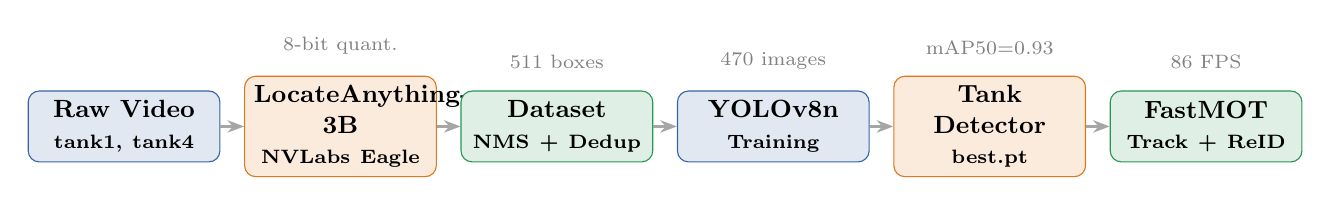
\begin{tikzpicture}[
  node distance=0.55cm and 0.3cm,
  box/.style={rectangle, rounded corners=4pt, draw=#1, fill=#1!15,
              text width=2.2cm, minimum height=0.9cm, align=center, font=\small\bfseries},
  arr/.style={-{Stealth[length=6pt]}, thick, color=gray!70}
]

\node[box=pipeblue]  (vid)   {Raw Video\\\scriptsize tank1, tank4};
\node[box=pipeorange, right=of vid]  (la)    {LocateAnything-3B\\\scriptsize NVLabs Eagle};
\node[box=pipegreen,  right=of la]   (ds)    {Dataset\\\scriptsize NMS + Dedup};
\node[box=pipeblue,   right=of ds]   (yolo)  {YOLOv8n\\\scriptsize Training};
\node[box=pipeorange, right=of yolo] (det)   {Tank Detector\\\scriptsize best.pt};
\node[box=pipegreen,  right=of det]  (mot)   {FastMOT\\\scriptsize Track + ReID};

\draw[arr] (vid)  -- (la);
\draw[arr] (la)   -- (ds);
\draw[arr] (ds)   -- (yolo);
\draw[arr] (yolo) -- (det);
\draw[arr] (det)  -- (mot);

\node[above=0.15cm of la,  font=\scriptsize, color=gray] {8-bit quant.};
\node[above=0.15cm of ds,  font=\scriptsize, color=gray] {511 boxes};
\node[above=0.15cm of yolo,font=\scriptsize, color=gray] {470 images};
\node[above=0.15cm of det, font=\scriptsize, color=gray] {mAP50=0.93};
\node[above=0.15cm of mot, font=\scriptsize, color=gray] {86 FPS};

\end{tikzpicture}
\end{center}

\vspace{0.3cm}
\begin{columns}[t]
\column{0.5\textwidth}
\textbf{Annotation} \\
\small Open-vocabulary VLM auto-labels tanks with no manual work
\column{0.5\textwidth}
\textbf{Tracking} \\
\small Kalman filter + KLT optical flow + PyTorch ReID
\end{columns}
\end{frame}

% ═══════════════════════════════════════════════════════════════════
\section{Data \& Annotation}
% ═══════════════════════════════════════════════════════════════════

\begin{frame}{Input Data}
\begin{columns}[T]
\column{0.5\textwidth}
\textbf{Video Sources}
\vspace{0.2cm}
\begin{itemize}
  \item \texttt{tank1.mp4} — 417 frames, 768$\times$432, 24 fps\\
        \textit{Side-view US Abrams, desert terrain}
  \vspace{0.2cm}
  \item \texttt{tank4.mp4} — 722 frames, 768$\times$432, 30 fps\\
        \textit{Aerial/drone view, multiple vehicles}
\end{itemize}
\vspace{0.4cm}
\textbf{Challenge} \\
\small Large domain gap between videos.
Aerial footage has vastly different appearance
from side-view footage.

\column{0.5\textwidth}
\begin{block}{Domain Distribution}
\small
\begin{tabular}{lll}
\toprule
Video & View & \# Vehicles \\
\midrule
tank1 & Side-angle & 1 \\
tank4 & Top-down   & 3+ \\
\bottomrule
\end{tabular}
\end{block}
\vspace{0.3cm}
\begin{alertblock}{Key Insight}
\small Training only on one domain fails on the other.
Both videos must be in the training set.
\end{alertblock}
\end{columns}
\end{frame}

% ─────────────────────────────────────────────────────────────────
\begin{frame}[fragile]{Auto-Annotation with LocateAnything-3B}
\begin{columns}[T]
\column{0.58\textwidth}
\textbf{LocateAnything} (NVLabs Eagle/Embodied)
\begin{itemize}
  \item 3B-parameter vision-language model
  \item Open-vocabulary: detect any class by text
  \item Outputs normalised box tokens \texttt{<box>x1 y1 x2 y2</box>}
  \item No fine-tuning needed — zero-shot detection
\end{itemize}

\vspace{0.3cm}
\textbf{Class prompts used}
\begin{itemize}
  \item \texttt{"military tank"}
  \item \texttt{"armored vehicle"}
  \item \texttt{"battle tank"}
\end{itemize}

\vspace{0.3cm}
\textbf{8-bit quantisation} \\
\small Loading with \texttt{load\_in\_8bit=True} reduces VRAM
from 8\,GB to 4.5\,GB, leaving room for inference on a 12\,GB GPU.

\column{0.42\textwidth}
\begin{block}{Annotation Script}
\begin{lstlisting}[language=bash]
python annotate_video_locate.py \
  --video tank1.mp4 \
  --classes "military tank" \
             "armored vehicle" \
             "battle tank" \
  --stride 1 \
  --min-area 0.0001 \
  --out dataset_tank1/
\end{lstlisting}
\end{block}

\begin{block}{Output Format (YOLO)}
\begin{lstlisting}
# class cx cy w h
0 0.572 0.645 0.237 0.294
\end{lstlisting}
\end{block}
\end{columns}
\end{frame}

% ─────────────────────────────────────────────────────────────────
\begin{frame}{Dataset Construction}
\begin{columns}[T]
\column{0.5\textwidth}
\textbf{Post-processing Steps}

\begin{enumerate}
  \item \textbf{Class collapse} \\
        \small All 3 class IDs (military tank, armored vehicle,
        battle tank) $\rightarrow$ class 0
  \vspace{0.2cm}
  \item \textbf{Second-stage NMS} \\
        \small Greedy IoU dedup with threshold 0.3.\\
        Removes overlapping boxes from different prompts
  \vspace{0.2cm}
  \item \textbf{Train/val split} \\
        \small 85\,\% train / 15\,\% val, random seed
  \vspace{0.2cm}
  \item \textbf{Multi-video merge} \\
        \small tank1 + tank4 combined for domain coverage
\end{enumerate}

\column{0.5\textwidth}
\begin{block}{Dataset Statistics}
\small
\begin{tabular}{lrr}
\toprule
Source     & Frames & Boxes \\
\midrule
tank1.mp4  & 350    & 350   \\
tank4.mp4  & 302    & 653   \\
\midrule
After NMS  & —      & \textbf{511}  \\
\midrule
Train set  & 367    & —     \\
Val set    & 103    & —     \\
\textbf{Total} & \textbf{470} & — \\
\bottomrule
\end{tabular}
\end{block}

\begin{exampleblock}{Box Reduction}
\small $1908 \rightarrow 511$ boxes after cross-prompt NMS
($-73\%$ duplicates removed)
\end{exampleblock}
\end{columns}
\end{frame}

% ═══════════════════════════════════════════════════════════════════
\section{YOLOv8 Training}
% ═══════════════════════════════════════════════════════════════════

\begin{frame}{YOLOv8 Training Strategy}
\begin{columns}[T]
\column{0.5\textwidth}
\textbf{Model: YOLOv8n}
\begin{itemize}
  \item 3M parameters, 8.2 GFLOPs
  \item Smallest YOLOv8 — fast inference on laptop GPU
  \item Pre-trained on COCO, fine-tuned on tank dataset
\end{itemize}

\vspace{0.3cm}
\textbf{Augmentation} (heavy, to compensate small dataset)
\begin{itemize}
  \item Mosaic 1.0, MixUp 0.1
  \item Rotation $\pm10°$, scale 0.5
  \item Horizontal flip 0.5
  \item HSV jitter (H: 0.015, S: 0.7, V: 0.4)
\end{itemize}

\column{0.5\textwidth}
\begin{block}{Training Configuration}
\small
\begin{tabular}{ll}
\toprule
Parameter   & Value \\
\midrule
Epochs      & 100 (early stop) \\
Image size  & 640$\times$640 \\
Batch size  & 16 \\
Optimiser   & AdamW (auto) \\
Patience    & 50 \\
Device      & RTX A3000 12\,GB \\
\bottomrule
\end{tabular}
\end{block}

\begin{exampleblock}{Results}
\small
\begin{tabular}{ll}
mAP50           & \textbf{0.935} \\
mAP50-95        & 0.811 \\
Precision       & 0.984 \\
Recall          & 0.851 \\
\end{tabular}
\end{exampleblock}
\end{columns}
\end{frame}

% ─────────────────────────────────────────────────────────────────
\begin{frame}{Iterative Domain Adaptation}
\begin{center}
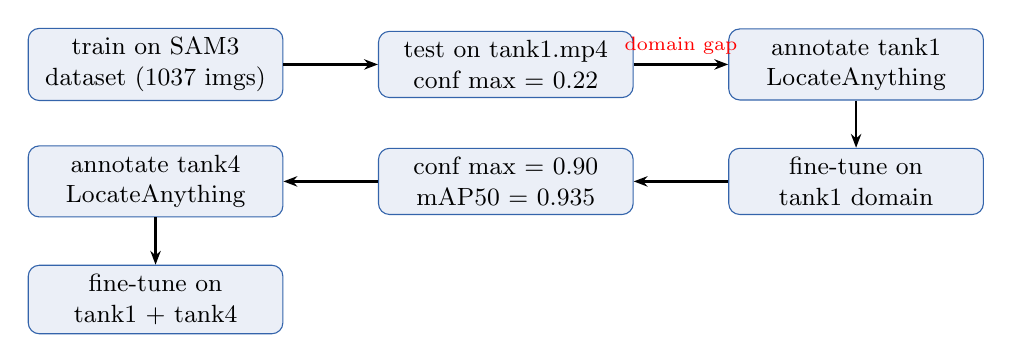
\begin{tikzpicture}[
  node distance=0.4cm,
  rnd/.style={rectangle, rounded corners, draw=pipeblue, fill=pipeblue!10,
              text width=3.0cm, minimum height=0.75cm, align=center, font=\small},
  arr/.style={-{Stealth[length=5pt]}, thick}
]

\node[rnd] (v1) {train on SAM3\\dataset (1037 imgs)};
\node[rnd, right=1.2cm of v1] (t1) {test on tank1.mp4\\conf max = 0.22};
\node[rnd, right=1.2cm of t1] (ann1) {annotate tank1\\LocateAnything};
\node[rnd, below=0.6cm of ann1] (v2) {fine-tune on\\tank1 domain};
\node[rnd, left=1.2cm of v2] (t2) {conf max = 0.90\\mAP50 = 0.935};
\node[rnd, left=1.2cm of t2] (ann4) {annotate tank4\\LocateAnything};
\node[rnd, below=0.6cm of ann4] (v3) {fine-tune on\\tank1 + tank4};

\draw[arr] (v1) -- (t1);
\draw[arr] (t1) -- node[above, font=\scriptsize, color=red]{domain gap} (ann1);
\draw[arr] (ann1) -- (v2);
\draw[arr] (v2)  -- (t2);
\draw[arr] (t2)  -- (ann4);
\draw[arr] (ann4) -- (v3);

\end{tikzpicture}
\end{center}
\vspace{0.2cm}
\small Each annotation round adds domain coverage.
The model progressively generalises from one video type to another.
\end{frame}

% ═══════════════════════════════════════════════════════════════════
\section{FastMOT Integration}
% ═══════════════════════════════════════════════════════════════════

\begin{frame}{FastMOT Architecture}
\begin{columns}[T]
\column{0.5\textwidth}
\textbf{FastMOT} is a multi-object tracker that combines:
\begin{enumerate}
  \item \textbf{Object Detector} — runs every $N$ frames
  \item \textbf{KLT Optical Flow} — tracks between detections
  \item \textbf{Kalman Filter} — motion prediction
  \item \textbf{Feature Extractor} — appearance ReID
  \item \textbf{Hungarian Association} — detection$\leftrightarrow$track matching
\end{enumerate}

\column{0.5\textwidth}
\begin{block}{Per-frame Decision}
\small
\begin{tabular}{ll}
\toprule
Frame type & Operation \\
\midrule
Frame 0          & Full detect + init  \\
Every $N$th frame & Detect + associate  \\
Other frames      & KLT flow only       \\
\bottomrule
\end{tabular}
\end{block}

\begin{alertblock}{Our modifications}
\small Replaced TRT-only detector and ReID with
PyTorch-native equivalents
\end{alertblock}

\end{columns}
\end{frame}

% ─────────────────────────────────────────────────────────────────
\begin{frame}[fragile]{Detector Integration: UltralyticsDetector}
\begin{columns}[T]
\column{0.55\textwidth}
\textbf{Problem:} FastMOT's built-in \texttt{YOLODetector} requires
a TensorRT-compiled engine (YOLOv4 format).

\vspace{0.2cm}
\textbf{Solution:} New \texttt{UltralyticsDetector} class that:
\begin{itemize}
  \item Wraps \texttt{ultralytics.YOLO(best.pt)}
  \item Implements FastMOT's async \texttt{Detector} ABC
  \item Runs inference in \texttt{detect\_async()}, caches result
  \item Returns \texttt{DET\_DTYPE} record array: \texttt{(tlbr, label, conf)}
  \item Includes second-stage greedy NMS (IoU $> 0.3$)
\end{itemize}

\column{0.45\textwidth}
\begin{block}{Detector Config (mot.json)}
\begin{lstlisting}
"detector_type": "ULTRALYTICS",
"ultralytics_detector_cfg": {
  "weights": "best.pt",
  "conf_thresh": 0.35,
  "iou_thresh": 0.25,
  "min_aspect_ratio": 0.1,
  "imgsz": 640
}
\end{lstlisting}
\end{block}
\begin{exampleblock}{Runtime}
\small 86 FPS on RTX A3000 12\,GB \\
Detector frame skip = 5
\end{exampleblock}
\end{columns}
\end{frame}

% ─────────────────────────────────────────────────────────────────
\begin{frame}[fragile]{ReID Integration: PyTorch Feature Extractor}
\begin{columns}[T]
\column{0.55\textwidth}
\textbf{Problem:} FastMOT's OSNet ReID uses TensorRT 7 API,
broken on TensorRT 10.

\vspace{0.2cm}
\textbf{Solution:} \texttt{TorchFeatureExtractor} using
\textbf{MobileNetV3-Small} backbone:
\begin{itemize}
  \item Pretrained on ImageNet (torchvision)
  \item Classifier head removed; 576-dim avgpool features
  \item L2-normalised embeddings
  \item Cosine distance for track association
  \item Graceful fallback chain:
        TRT $\rightarrow$ PyTorch $\rightarrow$ IoU-only
\end{itemize}

\column{0.45\textwidth}
\begin{block}{Feature Extractor}
\small
\begin{tabular}{ll}
\toprule
Property        & Value \\
\midrule
Backbone        & MobileNetV3-S \\
Embedding dim   & 576 \\
Distance metric & Cosine \\
Max ReID cost   & 0.85 \\
Track max age   & 150 frames \\
                & ($\approx$26\,s) \\
\bottomrule
\end{tabular}
\end{block}

\begin{block}{Startup log}
\begin{lstlisting}[language={}]
[INFO] PyTorch ReID
(MobileNetV3) loaded
— appearance matching
active
\end{lstlisting}
\end{block}

\end{columns}
\end{frame}

% ─────────────────────────────────────────────────────────────────
\begin{frame}[fragile]{Other Compatibility Fixes}
\begin{columns}[T]
\column{0.5\textwidth}
\textbf{Issues fixed}
\vspace{0.2cm}
\begin{itemize}
  \item \textbf{GStreamer auto-detect} \\
        \small \texttt{WITH\_GSTREAMER} hardcoded \texttt{True} \\
        $\rightarrow$ now reads \texttt{cv2.getBuildInformation()}
  \vspace{0.15cm}
  \item \textbf{Video codec} \\
        \small \texttt{avc1} requires HW encoder \\
        $\rightarrow$ fallback to \texttt{mp4v}, post-encode with \texttt{libx264}
  \vspace{0.15cm}
  \item \textbf{numba/coverage conflict} \\
        \small numba 0.65.1 needs \texttt{coverage $\geq$ 7.0}
  \vspace{0.15cm}
  \item \textbf{Label map} \\
        \small Class 0 showed as ``head'' (CrowdHuman) \\
        $\rightarrow$ pass \texttt{-l tank.names} at runtime
\end{itemize}

\column{0.5\textwidth}
\begin{block}{Wrapper Script (track\_tank.sh)}
\begin{lstlisting}[language=bash]
#!/bin/bash
# Activate venv, run FastMOT,
# re-encode to H.264
python app.py \
  -i "$INPUT" \
  -o "$TMP" \
  -l tank.names \
  -m

ffmpeg -i "$TMP" \
  -vcodec libx264 \
  -crf 23 -preset fast \
  "$OUTPUT" -y
\end{lstlisting}
\end{block}
\end{columns}
\end{frame}

% ═══════════════════════════════════════════════════════════════════
\section{Results}
% ═══════════════════════════════════════════════════════════════════

\begin{frame}{Detection \& Tracking Results}
\begin{columns}[T]
\column{0.5\textwidth}
\textbf{Detection Performance}
\begin{center}
\small
\begin{tabular}{lcc}
\toprule
Metric      & v1 (tank1) & v2 (merged) \\
\midrule
mAP50       & 0.995      & 0.935 \\
mAP50-95    & 0.872      & 0.811 \\
Precision   & 0.999      & 0.984 \\
Recall      & 1.000      & 0.851 \\
\midrule
Training imgs & 323      & 470   \\
\bottomrule
\end{tabular}
\end{center}
\small v1 = overfits single domain; v2 = generalises across domains

\column{0.5\textwidth}
\textbf{Tracking Performance}
\begin{center}
\small
\begin{tabular}{ll}
\toprule
Property          & Value \\
\midrule
Input resolution  & 1280$\times$720 \\
Detector skip     & 5 frames \\
Tracking FPS      & 86 (tank) \\
Confirm hits      & 3 frames \\
Duplicate thresh  & IoU $>$ 0.4 \\
Max track age     & 150 frames \\
ReID metric       & Cosine \\
\bottomrule
\end{tabular}
\end{center}
\end{columns}

\vspace{0.3cm}
\begin{exampleblock}{Confidence Distribution on Test Videos}
\small tank1.mp4: max=0.90, p75=0.72 \quad
       tank4.mp4: max=0.69, p75=0.44
\end{exampleblock}
\end{frame}

% ─────────────────────────────────────────────────────────────────
\begin{frame}{Pipeline Summary}
\begin{center}
\small
\begin{tabular}{lll}
\toprule
\textbf{Stage}       & \textbf{Tool / Model}          & \textbf{Key parameter} \\
\midrule
Frame extraction   & OpenCV + FFmpeg                & stride = 1 \\
Auto-annotation    & LocateAnything-3B (8-bit)      & 3 text prompts \\
NMS dedup          & Greedy IoU                     & threshold = 0.3 \\
Train/val split    & random seed 42                 & 85\,\% / 15\,\% \\
Detection model    & YOLOv8n (3M params)            & imgsz = 640 \\
MOT framework      & FastMOT                        & skip = 5 \\
Detector in MOT    & UltralyticsDetector            & conf = 0.35 \\
Between-frame      & KLT Optical Flow               & — \\
Motion model       & Kalman Filter                  & — \\
Appearance ReID    & MobileNetV3-Small (576-d)      & cosine, cost $\leq$ 0.85 \\
Output encoding    & libx264 (FFmpeg)               & CRF 23 \\
\bottomrule
\end{tabular}
\end{center}
\end{frame}

% ─────────────────────────────────────────────────────────────────
\begin{frame}{Limitations \& Future Work}
\begin{columns}[T]
\column{0.5\textwidth}
\textbf{Current Limitations}
\begin{itemize}
  \item Small training dataset (470 images)
  \item ReID struggles with partial visibility ($< 30\%$ in frame)
  \item MobileNetV3 not fine-tuned on tanks\\
        $\rightarrow$ generic ImageNet features
  \item No dedicated multi-camera support
\end{itemize}

\column{0.5\textwidth}
\textbf{Future Work}
\begin{itemize}
  \item \textbf{ReID fine-tuning} \\
        \small Extract per-ID crops from tracked video,
        train with triplet/ArcFace loss on tank identities
  \item \textbf{More data} \\
        \small Additional video domains, synthetic CARLA data
  \item \textbf{Larger detector} \\
        \small YOLOv8s/m for better small-object recall
  \item \textbf{Depth integration} \\
        \small Depth Anything v3 for 3-D track position
\end{itemize}
\end{columns}
\end{frame}

% ─────────────────────────────────────────────────────────────────
\begin{frame}{Conclusion}
\begin{block}{What was built}
A fully automated pipeline from raw video to tracked military vehicle output:
\end{block}

\vspace{0.3cm}
\begin{enumerate}
  \item \textbf{Zero-shot auto-annotation} via LocateAnything-3B
        (8-bit quantised, no GPU OOM)
  \item \textbf{Domain-adaptive training} across aerial and side-view footage
  \item \textbf{YOLOv8n} achieving mAP50 = 0.935 on merged dataset
  \item \textbf{FastMOT} with YOLOv8 detector, KLT flow, Kalman filter,
        and PyTorch ReID running at \textbf{86 FPS}
  \item \textbf{H.264 output} compatible with WhatsApp / mobile devices
\end{enumerate}

\vspace{0.3cm}
\begin{center}
\Large\textbf{Track any tank. Ship on WhatsApp.}
\end{center}
\end{frame}

\end{document}
